\chapter{Implementation} % The implementation should look at any issues you encountered as you tried to implement your design. During the work, you might have found that elements of your design were unnecessary or overly complex; perhaps third party libraries were available that simplified some of the functions that you intended to implement. If things were easier in some areas, then how did you adapt your project to take account of your findings? It is more likely that things were more complex than you first thought. In particular, were there any problems or difficulties that you found during implementation that you had to address? Did such problems simply delay you or were they more significant? You can conclude this section by reviewing the end of the implementation stage against the planned requirements.

@TODO - before this point, I still haven't mentioned use of Composer, AWS, and other tools, leaving my directory structure explanations a little bare. Also want to mention how my deployment script strips out tests etc from the zipped up, production-ready SmartResolution version
@TODO - describe in detail the models, data mappers and controller objects.
@TODO - make a SmartResolution style guide in the Wiki, pull in as an appendix
@TODO - improve SmartResolution developer instructions on Wiki, pull in as an appendix
@TODO - pull in module how-to guide documentation

\section{SmartResolution directory structure}

As the implementation followed an agile methodology, the design evolved over time and thus, the directory structure could not be determined up-front. Most (but not all) of the key directories and folders are outlined below:

\begin{minipage}{\textwidth}
\dirtree{%
.1 data/.
.1 features/.
.1 test/.
.1 vendor/.
.1 webapp/.
.2 core/.
.3 api/.
.3 controller/.
.3 db/.
.3 helpers/.
.3 model/.
.3 view/.
.2 modules/.
.3 other/.
.3 config.json.
.2 uploads/.
.2 index.php.
.2 routes.php.
.1 .travis.yml.
.1 composer.json.
.1 Gemfile.
}
\end{minipage}

\lstinline{data} contains fixture data for tests. This is also where the test and production SQLite3 databases reside.

\lstinline{features} contains the Cucumber features and Ruby step definitions.

\lstinline{test} contains all PHP unit tests.

\lstinline{vendor} is an automatically generated directory, created by Composer, containing all of SmartResolution's dependencies.

\lstinline{webapp/core} contains the core ODR platform, which uses an MVCR compound design pattern (\lstinline{webapp/routes.php} defines the routing component). The \lstinline{model}, \lstinline{view} and \lstinline{controller} directories are self-explanatory. I felt the need to separate the \lstinline{controller} and \lstinline{helpers} directories: the former contains controllers used by the routing (i.e. linking HTTP methods to application actions) whereas the latter contains general helper controllers available to both the higher-level routing controllers and the lower-level models.

Also inside the core is the \lstinline{db} directory, which contains middleware classes connecting the model classes to the database, since models should encapsulate the concept of whatever it is they are representing, rather than being responsible for the relational database to object mapping. This is discussed in detail later on in this section.

Finally, this folder also contains an \lstinline{api} directory, which defines all of the global functions available to modules. Having these in their own directory made generating module-specific API documentation easy.

Going back up a level, we have \lstinline{webapp/modules}, which contains any installed SmartResolution modules, such as the maritime collision module. A \lstinline{config.json} file (generated in a user-friendly way through the admin dashboard) denotes which modules are installed and whether or not they are active.

Finally, at the top level we have a few interesting files:

\lstinline{.travis.yml} - an instructions file for Travis Continuous Integration, describing how to set up the project and run its tests.

\lstinline{composer.json} - describes SmartResolution's dependencies. Developers can install all dependencies simply by running \lstinline{composer install}.

\lstinline{Gemfile} - describes SmartResolution's Ruby dependencies. Required for the Cucumber and Ruby integration tests.

\section{Routing}

\begin{figure}[h!]
  \centering
    \ifimages
    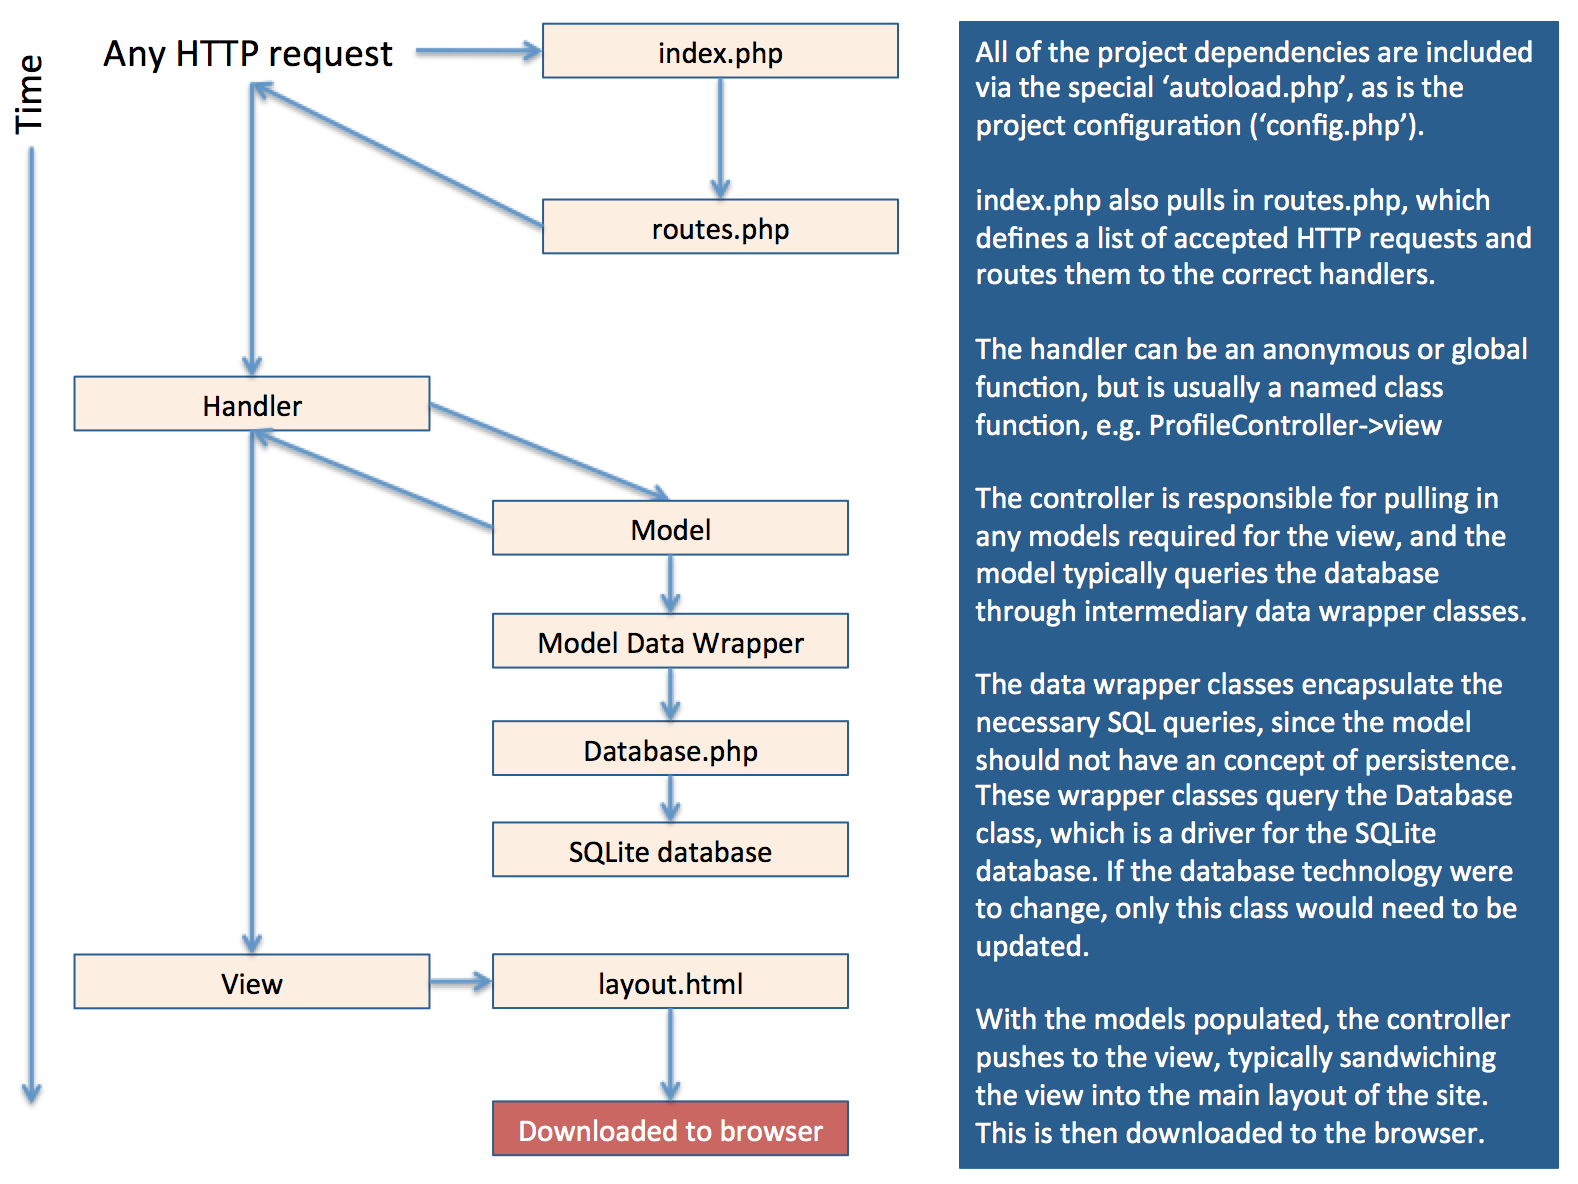
\includegraphics[width=\textwidth]{routing}
    \fi
  \caption{How SmartResolution processes HTTP requests}
  \label{uml:routing}
\end{figure}

Figure~\ref{uml:routing} shows how SmartResolution routes HTTP requests and renders data-driven pages. As described in the image, the HTTP request is processed by \lstinline{routes.php} and forwarded to the appropriate controller, which then instantiates the models and renders the view.

\section{Class diagrams}

The system was developed in an agile way, hence these class diagrams are not in the design section but the implementation section. What evolved from the design was a state pattern representing the current state of a dispute.

The class diagram in figure~\ref{uml:class} shows the classes in the \lstinline{webapp/core/model} directory, which encapsulate the business logic of the application.

\begin{figure}[h!]
  \centering
    \ifimages
    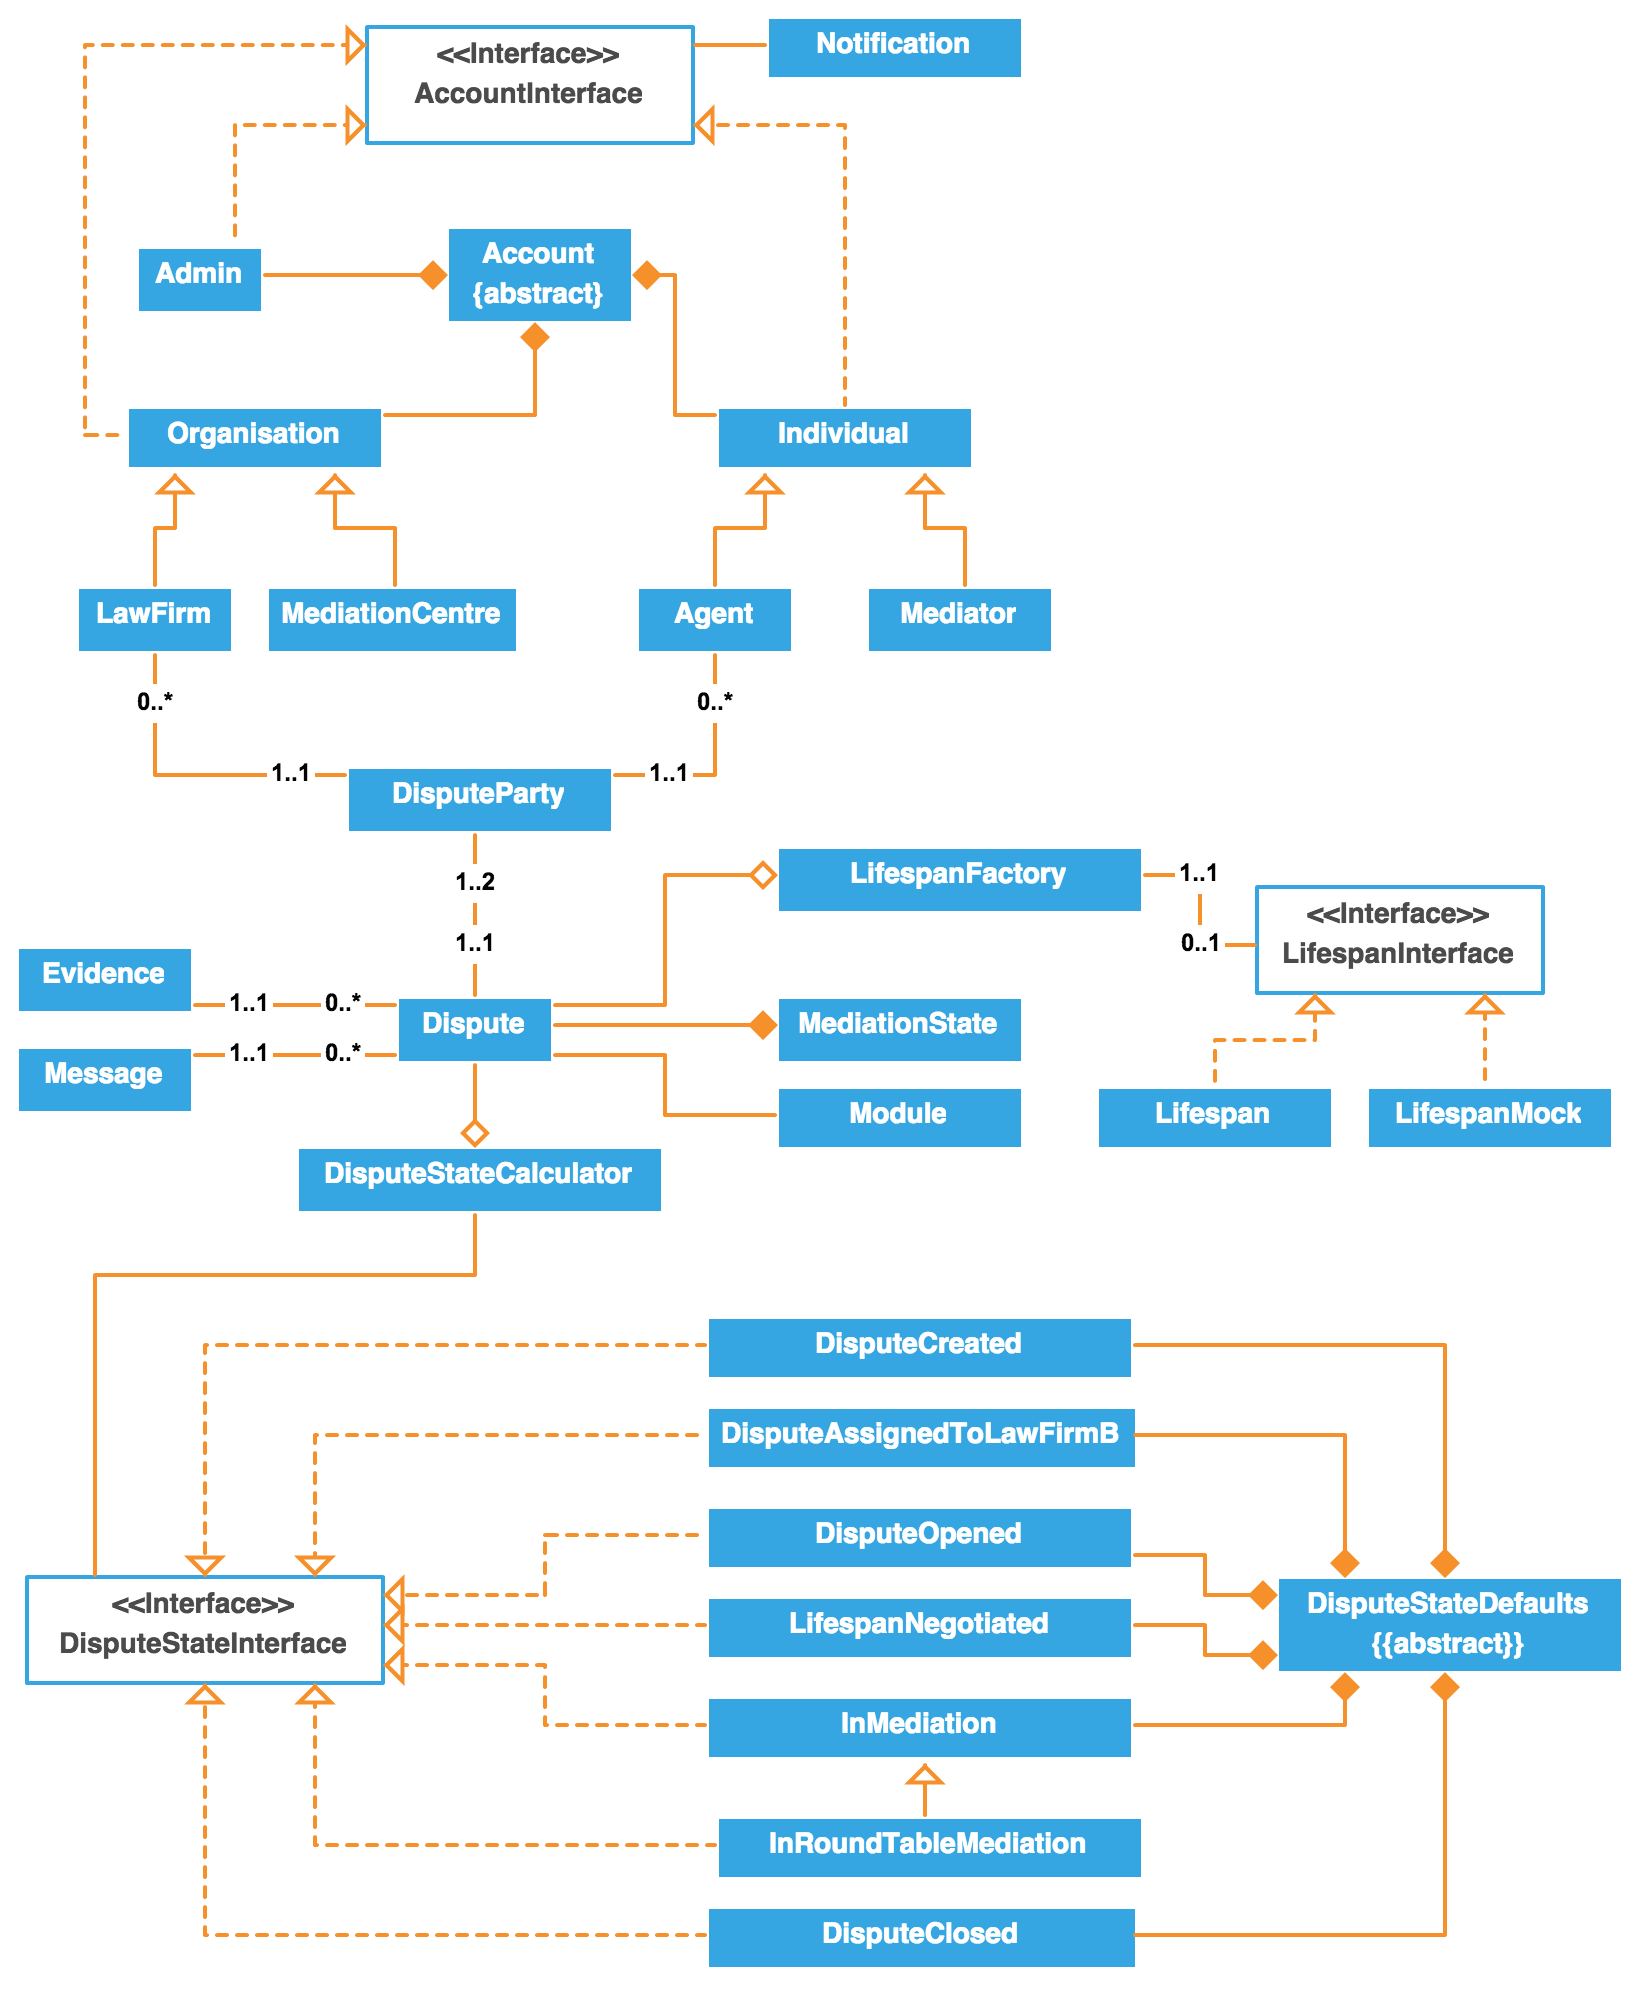
\includegraphics[width=\textwidth]{class}
    \fi
  \caption{Class diagram showing the model classes in SmartResolution}
  \label{uml:class}
\end{figure}

\subsection{Accounts}

Let's begin at the top of the figure: the \lstinline{AccountInterface}, which defines the core methods which all account types should define, whether the account is a law firm, a mediator or even an administrator. These methods include \lstinline{getEmail()}, \lstinline{getLoginId()}, \lstinline{__toString()} and so on.

Many of the methods in the interface will have the same implementation regardless of the account type. In these cases, the abstract class \lstinline{Account} defines the common implementations, but it does not implement the \lstinline{AccountInterface} interface since it cannot implement all of the methods for every account type.

The \lstinline{Organisation} and \lstinline{Individual} account types implement the \lstinline{AccountInterface} interface and extend the \lstinline{Account} abstract class to further define any missing function definitions specific to their own account type. Finally, the specialised subclasses inherit from \lstinline{Organisation} or \lstinline{Individual} and override or call parent function definitions where necessary.

\subsection{Disputes}

Every fully instantiated dispute has two dispute parties which comprises of a law firm, an agent and a dispute summary. A dispute can have zero-to-many items of evidence (uploaded by the agents) associated with it and zero-to-many messages sent back and forth between the agents. Every dispute should also have a lifespan, but this is more complicated than it might first appear so is discussed in further detail in the next subsection.

A dispute's \emph{type} denotes whether or not a module is pulled in to expand the options available to it. By default, all disputes are of type `Other', but this is where our maritime collision logic would come into play. With the maritime collision module activated, agents have the option to change the dispute type to `Maritime Collision', thereby unlocking the AI that the module offers.

Finally, disputes have a \emph{mediation state}: that is, a dispute may or may not be in mediation. A dispute may also be somewhere in between, e.g. the agents have decided upon a mediation centre but not yet chosen a mediator. This is all encapsulated in the MediationState class.

\subsection{Lifespans}

Every dispute should have a lifespan. This becomes somewhat complicated, since a lifespan can be proposed by either party, must be agreed by both parties, must only be applied between the start and end points of a lifespan, and can be renegotiated at any time.

With this in mind, every dispute can be said to have two lifespans: the `current' and `latest' lifespans. Figure~\ref{uml:lifespan} highlights the difference between the two. 

\begin{figure}[h!]
  \centering
    \ifimages
    
\includegraphics[width=\textwidth]{lifespan}
    \fi
  \caption{Visualisation showing the difference between the `current' and `latest' lifespans}
  \label{uml:lifespan}
\end{figure}

The `current' lifespan is the most recent accepted Lifespan that has been attributed to the given dispute. If no Lifespan has been accepted, this retrieves the most recent \emph{offered} Lifespan. If no Lifespan has even been offered, this returns a mock Lifespan object so that all of the lifespan-related method calls still work, to save us complicating our dispute object.

For most purposes, the `current' lifespan is what is required. This is the lifespan that has generally been agreed by both parties and is used for checking if a dispute is still ongoing before allowing an agent to send a message, for example.

The `latest' lifespan ignores whether or not a lifespan has been accepted and retrieves the very latest lifespan proposal. This is required in special cases, such as in the rendering of the lifespan on the dispute dashboard, to highlight the fact that a new lifespan has been proposed and it needs to be accepted or declined.

\subsection{Dispute State}

Separately from the `mediation state' is the higher level dispute state. A dispute is in a different state depending on whether or not all agents have been assigned, a lifespan has been negotiated, and so on. The state of the dispute dictates what actions are available to the parties involved.

In early versions of the project, the codebase began to get quite messy because classes throughout the system would examine a dispute's state to decide whether or not they could perform some action. This led to complicated \lstinline{if} statements, like the one below:

\begin{lstlisting}
if ($dispute->state() === 'Open' || $dispute->state() === 'InMediation' || $dispute->state() === 'NegotiatingLifespan') {
    doSomething();
}
\end{lstlisting}

Figure~\ref{uml:states} shows how the state pattern was adopted to overcome problems like this. Classes throughout SmartResolution could now query the dispute's state directly, as the responsibility of whether or not an action could be performed was encapsulated inside the state itself. The above example could thus be rewritten as follows:

\begin{lstlisting}
if ($dispute->state()->canDoSomething()) {
    doSomething();
}
\end{lstlisting}

\begin{figure}[h!]
  \centering
    \ifimages
    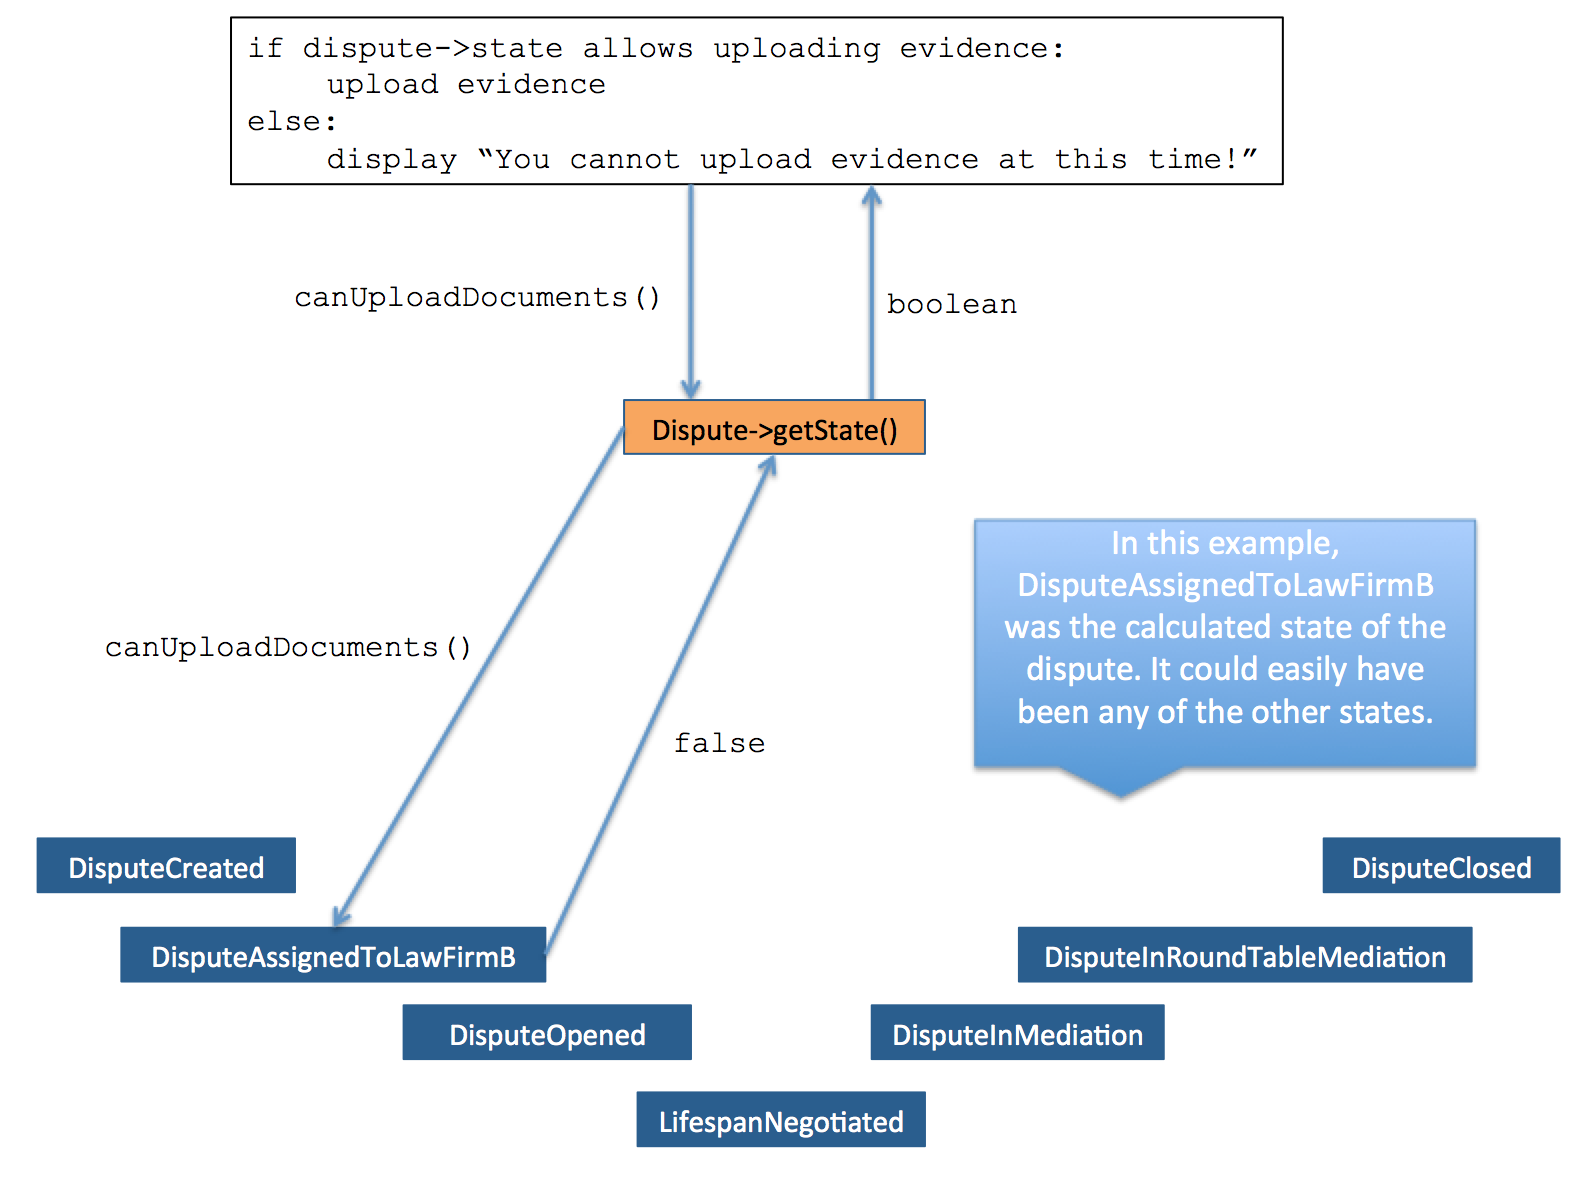
\includegraphics[width=\textwidth]{states}
    \fi
  \caption{Visualisation of how the state pattern works in SmartResolution}
  \label{uml:states}
\end{figure}

The list of possible states are as follows:

\begin{itemize}
    \item \textbf{DisputeCreated} - this is the very first state of the dispute and represents a dispute that has just been created. At this stage, the first dispute party is complete (it will have a law firm and an agent associated with it), but it has not been opened against another law firm.
    \item \textbf{DisputeAssignedToLawFirmB} - this represents the state of the dispute when it has just been assigned to the other law firm. At this stage, one dispute party is complete, whilst the other only has the law firm. We are still waiting for the law firm to assign an agent.
    \item \textbf{DisputeOpened} - all law firms and agents have been assigned. Now a lifespan must be negotiated.
    \item \textbf{LifespanNegotiated} - the agents have managed to negotiate a lifespan and there is nothing more to do to initiate the dispute. When the start date is surpassed, the dispute is underway and the agents are free to perform all dispute-related actions. When the end date passes, the dispute is automatically closed.
    \item \textbf{DisputeInMediation} - the agents have decided to put the dispute into mediation and have negotiated a mediation centre and a mediator. It is important to note that not all disputes will necessarily reach this stage.
    \item \textbf{DisputeInRoundTableMediation} - the dispute is in mediation, but all parties are free to communicate openly. By default, a dispute in mediation disables direct communication between the two agents. The mediator can enable round-table communication to put the dispute into this state.
    \item \textbf{DisputeClosed} - the dispute is now closed, either because an agent closed it or because the lifespan of the dispute came to an end. It may have been closed successfully (the dispute was resolved) or unsuccessfully (the dispute had to be resolved by other means, e.g. court).
\end{itemize}

As can be seen in the class diagram in figure~\ref{uml:class}, most of these states inherit from the DisputeStateDefaults class, which defines the default permissions regarding dispute actions and means we don't have to specify long lists of true/false values where only one or two items may have changed between states. The exception to this rule is the \lstinline{InRoundTableMediation} state, which is only very slightly different to the \lstinline{InMediation} state and thus extends that class rather than the default class.

\section{Comments}

@TODO mention this somewhere:

The codebase is liberally commented throughout, using API-style markup. This was a difficult decision, discussed and justified in appendix~\ref{appendix:comments}.

\section{SmartResolution Marketplace}

The SmartResolution website was developed locally using many of the same technologies as the core SmartResolution software, including F3, Bootstrap, Composer and so on. For the SmartResolution Marketplace functionality to be implemented, it was clear that the website would need to be deployed somewhere remotely.

\subsection{Choosing a server}

A locally configured, physical server would not be practical for hosting the SmartResolution marketplace. If ever the platform became popular, it would not be able to cope with the numbers of people downloading the software (which weighs in at over 400KB) and browsing the documentation. Moreover, it is an unnecessary maintenance and upfront expense when so many alternatives exist.

Cloud computing as a web hosting service is becoming increasingly popular [REF], Amazon Web Services (AWS) chief amongst these in terms of exponential growth, being utilised by companies big and small, including the BBC. [REF] Its popularity is down to its speed and scalability, as well as the low cost to market.

AWS has server farms in X, Y and Z, making it possible to make optimised regional sites, content delivery networks (CDNs) and so on. It can be configured to automatically deploy additional EC2 (Amazon Elastic Compute Cloud) instances when there is a surge in website traffic, to cope with surges in demand.

Other alternatives exist, of course, such as Unlimited Web Hosting [REF], which is a cloud web hosting service I like to use for my personal projects. However, SmartResolution requires shell access for the installation process, in order to download dependencies through Composer, set up the SQLite database and so on.

Unlike Unlimited Web Hosting, AWS provides root access, and though other services also provide this facility (DigitalOcean, for example [REF]), it made sense to invest time in configuring an infrastructure that would be able to cope with increases in traffic should SmartResolution ever require it.

\subsection{Configuring the server}

At the point where an EC2 instance is started, a dynamic IP address is generated, making the instance available at that given IP. By default, that IP address is not persistent and every 24 hours or so the IP addresses are reallocated and the instance must be reached through a different IP.

AWS offers an `Elastic IP' facility, which allows you to generate a permanent IP address and allocate it to an EC2 instance. This costs a little extra but is a necessary step to ensure the website is always locatable.

Finally, Amazon's Route 53 service is a scalable DNS and allows you to link a domain/subdomain name to an IP address, so that browsers querying that domain name are redirected to the content at the IP address endpoint.

smartresolution.org was purchased through the domain registrar gandi.net [REF] and the nameservers for Amazon's Route 53 service were specified as the DNS. On the server itself, the EC2 instance is automatically deployed as a LAMP server running Amazon's own Linux [REF], Apache, MySQL and PHP.
%http://aws.amazon.com/amazon-linux-ami/

The decision was made to separate the two concepts of the SmartResolution software and the SmartResolution website, so a live demo of the software should be available on a subdomain rather than the main site index.

To accomplish this, a VirtualHost was specified in the Apache configuration to redirect any requests for demo.smartresolution.org to a specific demo folder containing the SmartResolution software, which could be easily updated independent of SmartResolution website updates.

All of this is demonstrated in figure~\ref{uml:serverConfig}.

\begin{figure}[h!]
  \centering
    \ifimages
    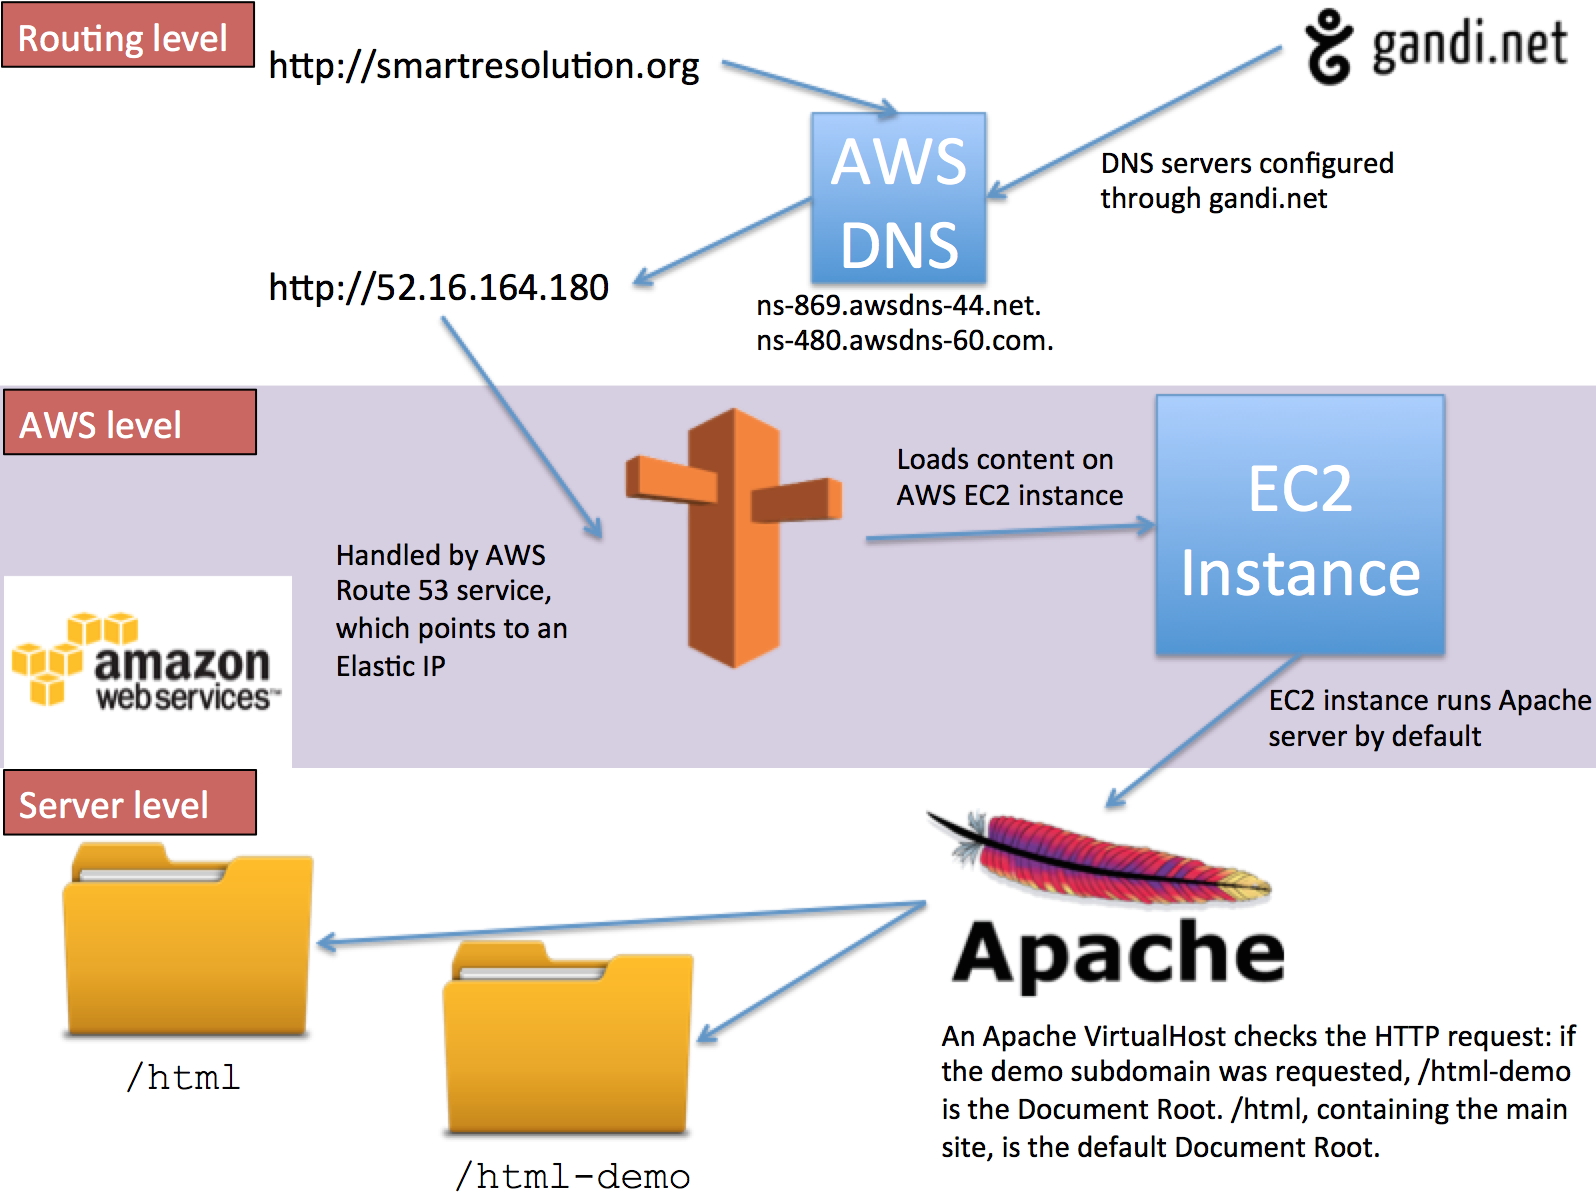
\includegraphics[width=\textwidth]{server_config}
    \fi
  \caption{The server configuration for smartresolution.org}
  \label{uml:serverConfig}
\end{figure}

\subsection{Continuous deployment}

Though continuous integration is important for ensuring that the codebase remains fully functional, continuous deployment is important for ensuring that the version of SmartResolution available for demo and for download on the SmartResolution website is fully up to date. It needed to be simple to keep both elements at the latest version, and everything ought to be as automated as possible.

I wrote a bash script specific to the SmartResolution vendor site which clears the html and html-demo folders outlined in figure~\ref{uml:serverConfig}, then re-downloads and installs the website and the software from the website repository and the software repository respectively. The script calls PHPDoc to generate the SmartResolution core API documentation and module documentation, and the script also strips out unnecessary files such as tests and Travis configuration before zipping up the file as a production-ready download.

In an ideal world, this script would be triggered via a Git web hook [REF] so that the website, demo and download file are all updated whenever an update is pushed to either the website or software repository. However, triggering this bash script through PHP is a security issue and is made very difficult to accomplish through AWS' default Apache and PHP configuration. After some failed attempts and with time pressing on, it was decided that manually signing into the EC2 instance and running the update script was not too much of an inconvenience.

The script can be found at appendix X @TODO?? (this will be part of the technical hand-in so perhaps isn't needed here)